\documentclass[tikz,border=3.14mm]{standalone}
\usetikzlibrary{decorations.markings,arrows.meta,bending}

\begin{document}
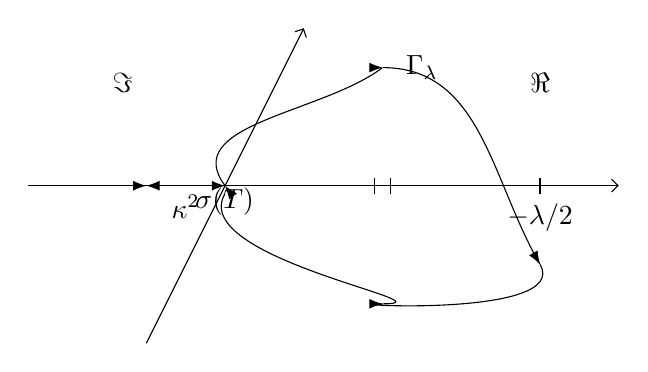
\begin{tikzpicture}[
    arrow inside/.style = {postaction={decorate},decoration={markings,
        mark=at position 0 with {\arrow{Latex[bend]}}},shorten >=0.2pt},
    >={Straight Barb[bend]}
]

% axis
\draw[->] (-1.5,0) -- (6,0) coordinate (xaxis);
\draw[->] (0,-2) -- (2,2) coordinate (yaxis);

% spectrum of T
\draw[dashed] (0,0) -- node[below] {$\kappa^2$} (1,0);
\draw[dashed,right] (0.5,-0.2) node {$\sigma(T)$};

% contours
\draw[arrow inside] (0,0) -- (1,0);
\draw[arrow inside,bend right=30] (1,0) to[out=90,in=180] (3,1.5);
\draw[arrow inside] (3,1.5) to[out=0,in=120] (5,-1);
\draw[arrow inside] (5,-1) to[out=-60,in=180] (3,-1.5);
\draw[arrow inside] (3,-1.5) to[out=0,in=-120] (1,-0.1);

% labels
\draw (5,0.1) -- (5,-0.1) node[below] {$-\lambda/2$};
\node at (5,1.3) {$\Re$};
\node at (-0.3,1.3) {$\Im$};
\draw (2.9,0.1) -- (2.9,-0.1) node[below] {};
\draw (3.1,0.1) -- (3.1,-0.1) node[below] {};
\node at (3.1,0.1) [above right] {};
\path (3,0) node[below] {};
\draw[arrow inside] (0,0) -- (-0.1,0) node[above left] {};
\path (1,0) node[below] {};
\draw[arrow inside] (1,0) -- (1.1,0);

% contour name
\node at (3.5,1.5) {$\Gamma_\lambda$};

\end{tikzpicture}
\end{document}